\section{Experimental Evaluation}
\label{sec:evaluation}

We evaluate our Gdev prototype, using the Rodinia
benchmarks~\cite{Che_IISWC09}, GPU-accelerated eCryptfs encrypted
filesystem from KGPU~\cite{Sun_SECURITY11_Poster}, FAST database
search~\cite{Kim_SIGMOD10}, and some dataflow
microbenchmarks from PTask~\cite{Rossbach_SOSP11}.
We disclose that the basic performance of our prototype is practical
even compared to proprietary software, and also demonstrate that Gdev
provides significant benefits for GPU applications in time-sharing
systems.

Our experiments are conducted with the Linux kernel 2.6.39 on NVIDIA
GeForce~GTX~480 graphics card and Intel Core~2~Extreme QX9650 processor.
GPU programs are written in CUDA and compiled by NVCC~\cite{CUDA40},
while CPU programs are compiled by gcc 4.4.6.

\subsection{Basic Performance}

We first investigate the basic performance of standalone applications achieved
by our Gdev prototype compared to NVIDIA's proprietary driver and
library~\cite{BLOB,CUDA40}, in order to argue that the rest of our
evaluation is practical in the real world. 
To do so, we need to determine what resource parameters maximize
performance for our Gdev prototype.
Figure~\ref{fig:chunk} shows the impact of the chunk size on memory-copy
DMA speeds for both host-to-device (HtoD) and device-to-host (DtoH)
data transmissions, tested by different data sizes.
The throughput is affected by overhead when the chunk size is small,
while it is also affected by blocking times when the chunk size is
large.
One may observe that a chunk size of 4MB seems to be the best trade-off
for both HtoD and DtoH.
Figure~\ref{fig:io_access} depicts the relative speed of direct I/O
access to DMA for a small size of data. 
Due to some cache effects, HtoD and DtoH behave in a different manner.
According to the results, the data transfer speeds inverse around a
data size of 4KB for HtoD and 1KB for DtoH.
Henceforth, we set the chunk size to 4MB and the data size boundary of
direct I/O access to 4KB for HtoD and 1KB for DtoH, based on the above
results. 

Figure~\ref{fig:memcpy} demonstrates the memory-copy throughts achieved
by our Gdev prototype compared to NVIDIA's proprietary software.
``Gdev/User'' represents a version of Gdev that employs a runtime
library in the user-space, while ``Gdev'' represents the one ingetrating
the runtime support into the OS.
Interestingly, the user-space runtime achieves higher throughputs than
the OS runtime especially for DtoH.
We found that this difference is due to host-to-host \texttt{memcpy}
effects.
In particular, \texttt{memcpy} in the Linux kernel performs slower than
that in the user-space GNU library when copying data from the I/O memory
to the main memory.
We claim that this would be a disadvantage of integrating the runtime
support into the OS, but an in-depth investigation is required.
Apart from DtoH with the OS runtime, our Gdev prototype and the
proprietary software are almost competitive.
This explains that we could identify how to optimize memory-copy
operations for the GPU.
 
\begin{figure}[t]
 \begin{center}
  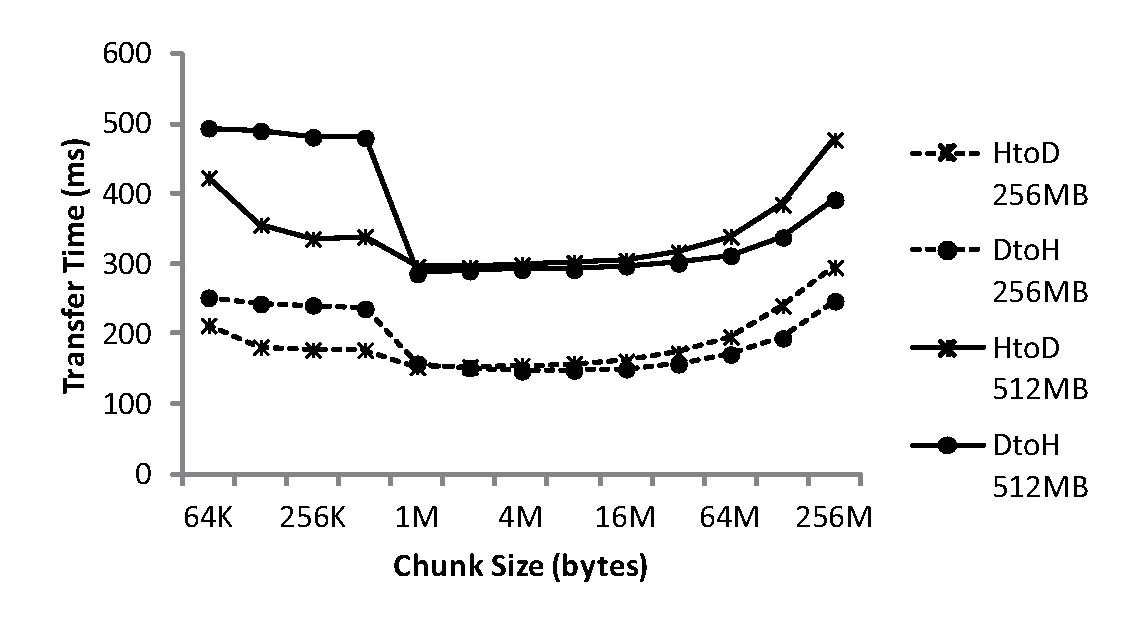
\includegraphics[width=0.8\hsize]{eps/chunk.eps}\\
  \vspace{-1.5em}
  \caption{Impact of the chunk size on DMA speeds.}
  \label{fig:chunk}
 \end{center}
 \begin{center}
  \vspace{-0.5em}
  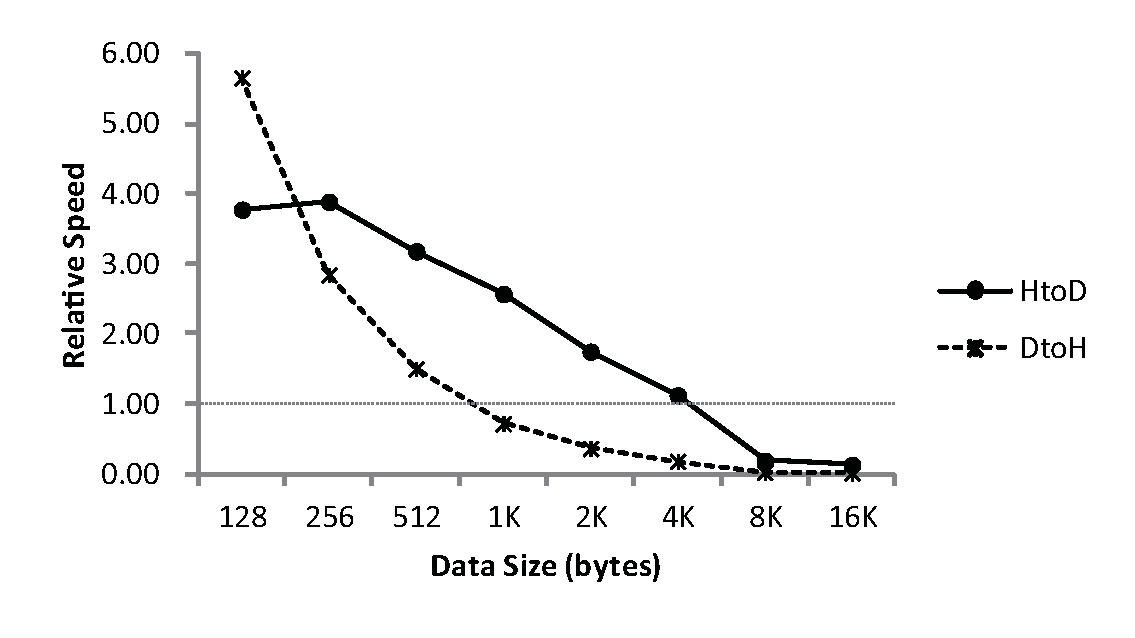
\includegraphics[width=0.8\hsize]{eps/dma.eps}\\
  \vspace{-1.5em}
  \caption{Relative speed of I/O access to DMA.}
  \label{fig:io_access}
 \end{center}
 \begin{center}
  \vspace{-0.5em}
  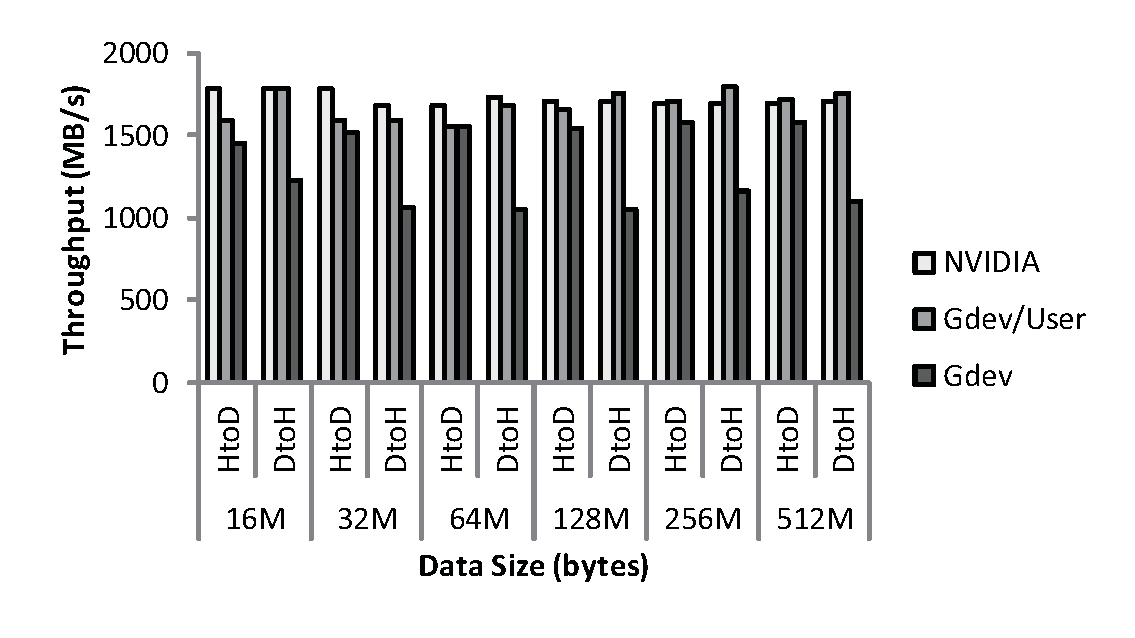
\includegraphics[width=0.9\hsize]{eps/memcpy.eps}\\
  \vspace{-1.5em}
  \caption{Memory-copy performation.}
  \label{fig:memcpy}
 \end{center}
 \vspace{-2em}
\end{figure}

\begin{table}[t]
 \caption{List of benchmarks.}
 \label{tab:benchmarks}
 \begin{center}
  {\footnotesize
  \begin{tabular}{|l|l|}
   \hline
   \textbf{Benchmarks} & \textbf{Description}\\
   \hline
   LOOP & Long-loop compute without data \\
   \hline
   MADD & 1024x1024 matrix addition\\
   \hline
   MMUL & 1024x1024 matrix multiplication\\
   \hline
   CPY & 256MB of HtoD and DtoH\\
   \hline
   PINCPY & CPY using pinned host I/O memory\\
   \hline
   BP & Back propagation (pattern recognition)\\
   \hline
   BFS & Breadth-first search (graph algorithm)\\
   \hline
   HW & Heart wall (medical imaging)\\
   \hline
   HS & Hotspot (physics simulation)\\
   \hline
   LUD & LU decomposition (linear algebra)\\
   \hline
   NN & K-nearest neighbors (data mining)\\
   \hline
   NW & Needleman-wunsch (bioinformatics)\\
   \hline
   SRAD & Speckle reducing anisotropic diffusion (imaging)\\
   \hline
   SRAD2 & SRAD with random pseudo-inputs (imaging)\\
   \hline
  \end{tabular}
  }
 \end{center}
\vspace{-1.5em}
\end{table}

Figure~\ref{fig:basic_performance} demonstrates the standalone
benchmarking results achieved by our Gdev prototype compared to the
proprietary software, using our microbenchmarks and the Rodinia
benchmarks listed in Table~\ref{tab:benchmarks}.
First of all, we found that GeForce GTX 480 has ``performance mode'' to
boost computing performance, which we have not yet figured out how to
turn on.
As observed in LOOP, our open-source implementation inevitably incurs
about 20\% of decrease in computing performance compared to the
proprietary software.
However, the impact on application performance depends on workloads.
If the workload is very compute-intensive, such as HW and SRAD, the
impact appears to be high, while some friendly workload, such as BFS and
HS, hides the impact.
In either case, we claim that this performance demerit comes from our
open-source solution, attributed to the fact that the architectural
specification is not open to the public, but does not limit the concept
of Gdev.
These benchmarks also identify that our runtime-unified OS approach
would not be appreciated by data-intensive workloads.
For example, BP deals with a very large size of data, while its compute
demand is not very high.
Such a workload faces performance degradation with our Gdev prototype
due to the slow host-to-host \texttt{memcpy} operation in the OS, as
discussed above.
PINCPY, on the other hand, exhbits a very little difference in
performance, since it does not need the host-to-host \texttt{memcpy}
operation.

\begin{figure}[t]
 \begin{center}
  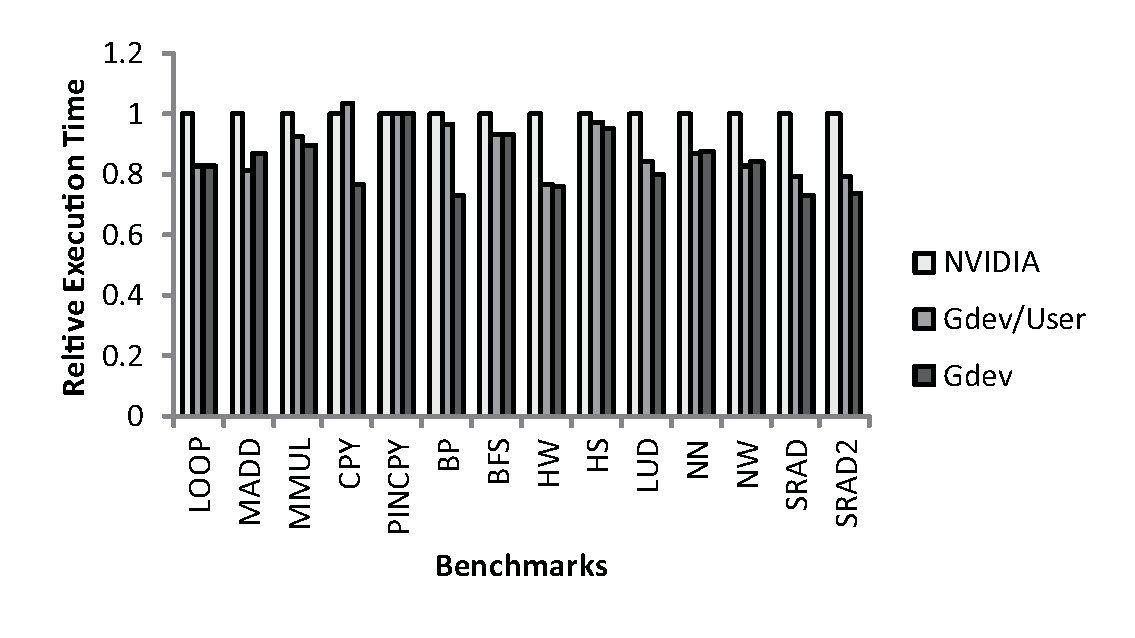
\includegraphics[width=0.9\hsize]{eps/basic_performance.eps}\\
  \vspace{-1.5em}
  \caption{Basic standalone performance.}
  \label{fig:basic_performance}
 \end{center}
 \vspace{-1.5em}
 \begin{center}
  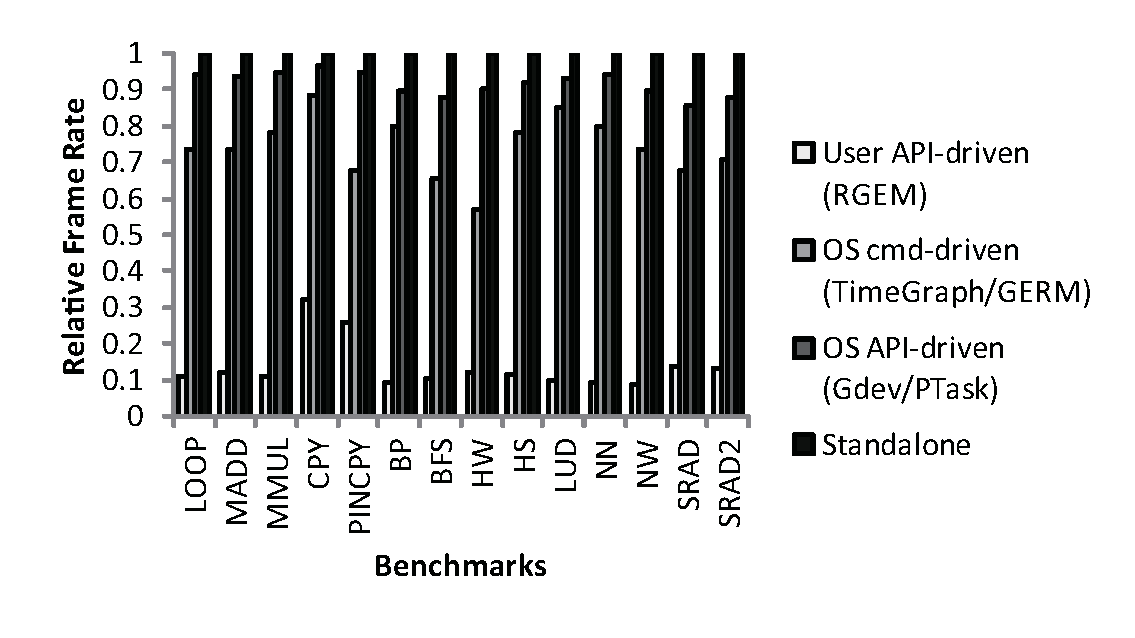
\includegraphics[width=0.9\hsize]{eps/scheduler_overhead.eps}\\
  \vspace{-1.5em}
  \caption{Unconstrained real-time performance under extreme workloads.}
  \label{fig:scheduler_overhead}
 \end{center}
  \vspace{-1.5em}
\end{figure}

\subsection{Reliability}

We next investigate the reliability of GPU schedulers, comparing the OS
API-driven scheme adopted by Gdev and PTask~\cite{Rossbach_SOSP11}, OS
command-driven scheme adopted by TimeGraph~\cite{Kato_ATC11} and
GERM~\cite{Bautin_MCNC08}, and user-space API-driven scheme adopted by
RGEM~\cite{Kato_RTSS11}.
We execute each Rodinia benchmark recursively as fast as possible in
real-time together with such workloads representing malicious programs
that launch many meaningless GPU commands bypassing the runtime library.
The user-space API-driven scheduler severely suffers from this
situation, since it cannot schedule such workloads that bypass the
scheduler itself.
The OS command-driven scheduler can limit the influence of these
workloads by scheduling commands, but it still incurs some overhead to
schedule them.
The OS API-driven scheduler, on the other hand, can simply reject such
workloads, since they are not submitted using the API.
Gdev and PTask are both API-driven, but PTask exposes the scheduler
system call to the user space, such as \texttt{sys\_set\_ptask\_prio},
which could allow misbehaving applications to jeopardize the scheduler.
As a consequence, we believe that Gdev is more reliable than previous
schemes.

\subsection{GPU Acceleration for the OS}

\begin{figure}[t]
 \begin{center}
  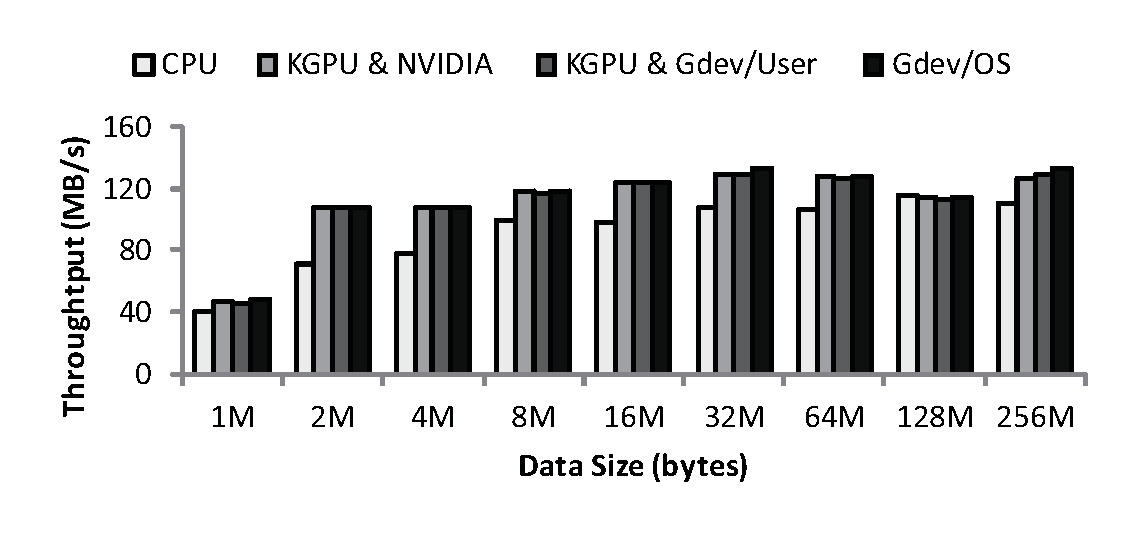
\includegraphics[width=0.9\hsize]{eps/ecryptfs_read.eps}\\
  \vspace{-1.5em}
  \caption{Read throughput of eCryptfs.}
  \label{fig:ecryptfs_read}
 \end{center}
 \vspace{-1.5em}
 \begin{center}
  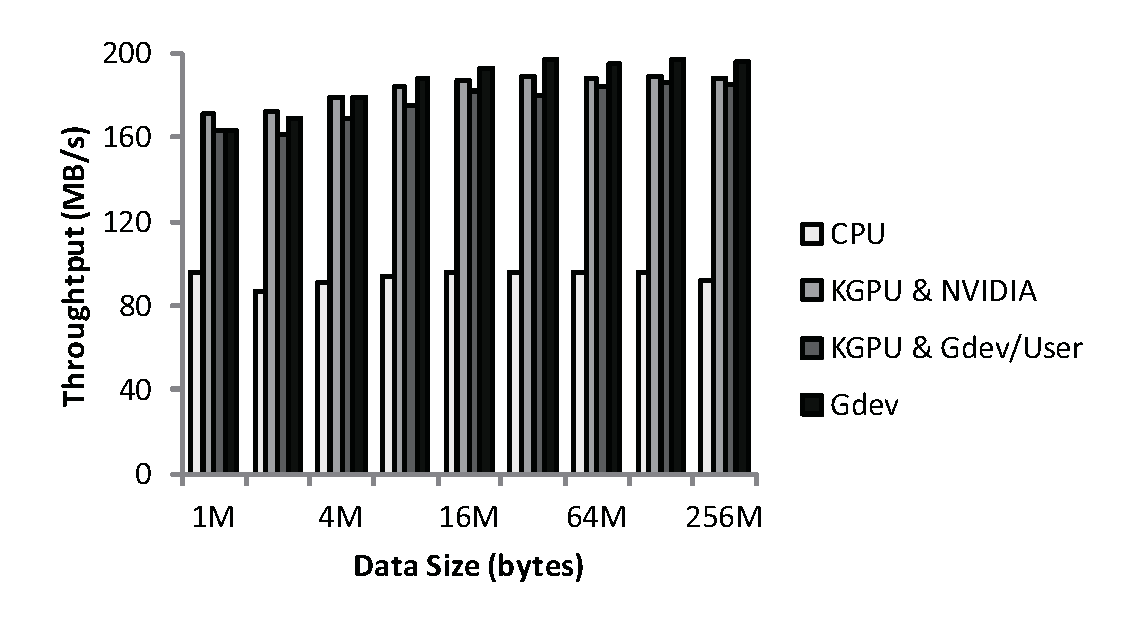
\includegraphics[width=0.9\hsize]{eps/ecryptfs_write.eps}\\
  \vspace{-1.5em}
  \caption{Write throughput of eCryptfs.}
  \label{fig:ecryptfs_write}
 \end{center}
 \vspace{-1.5em}
 \begin{center}
  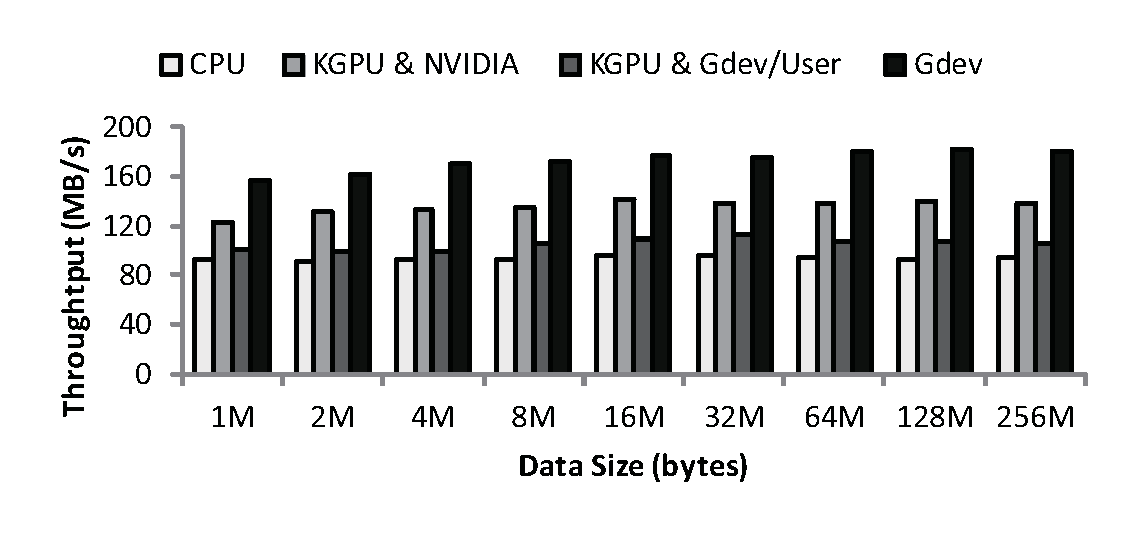
\includegraphics[width=0.9\hsize]{eps/ecryptfs_write_multitask.eps}\\
  \vspace{-1.5em}
  \caption{Write throughput of eCryptfs in mult-tasking.}
  \label{fig:ecryptfs_write_multitask}
 \end{center}
 \vspace{-1.5em}
\end{figure}

We now evaluate the GPU acceleration for the Linux encrypted filesystem,
using KGPU's implementation of eCryptfs~\cite{Sun_SECURITY11_Poster}.
KGPU is a framework that allows the OS to access the user-space runtime
library to use the GPU for its computations.
We have modified KGPU's eCryptfs to call the CUDA API functions
provided by Gdev directly, instead of sending requests to the KGPU user-space
daemon.
Figure~\ref{fig:ecryptfs_read} and \ref{fig:ecryptfs_write} show the
read and write throughputs of several versions of eCryptfs.
``CPU'' represents the CPU implementation, while ``KGPU \& NVIDIA'' and
``KGPU \& Gdev/User'' represent those that use KGPU with NVIDIA's
library and Gdev's library in the user space respectively.
``Gdev'' is our solution that enables the eCryptfs module to use the GPU
directly in the OS.
Due to some page cache effects, the read and write throughputs are not
identical, but the advantage of using the GPU is clearly observed.
One can also observe that our runtime-unified OS approach does not
provide sufficient performance improvements over KGPU's user-space
approach.
However, this is reasonable because a magunitude of improvements in
latency achieved by our OS approach would be at most microseconds, while
the AES/DES operations of eCryptfs performed on the GPU are
orders-of-miliseconds.
Nonetheless, Gdev is fairly beneficial in that OS applications do not need
to depend on the user-space library.

A further benefit of using Gdev for OS applications appears in
multi-tasking environments.
Figure~\ref{fig:ecryptfs_write_multitask} shows the write throughputs of
eCryptfs when the FAST search task~\cite{Kim_SIGMOD10} is competing
the GPU in the background.
Since Gdev supports priorities, we assign eCryptfs the highest priority,
while the FAST task is also assigned a higher priority than other tasks.
What happens in this scenario is that the performance of eCryptfs is
affected by the FAST task without a priority scheme, as observed in
``KGPU \& NVIDIA''.
Even with priorities, KGPU could still suffer from a priority inversion
problem where the high-priority eCryptfs task is reduced to the priority
level of the KGPU daemon when accessing the GPU, while the FAST task is
running at a higher-priority level than the daemon.
We can assign a high priority to the KGPU daemon, but it affects all
user-space GPU applications.
Using Gdev, on the other hand, GPU applications execute at the identical
priority level, which avoids such a priority inversion.

\subsection{Impact of Shared Memory}

\begin{figure}[t]
 \begin{center}
  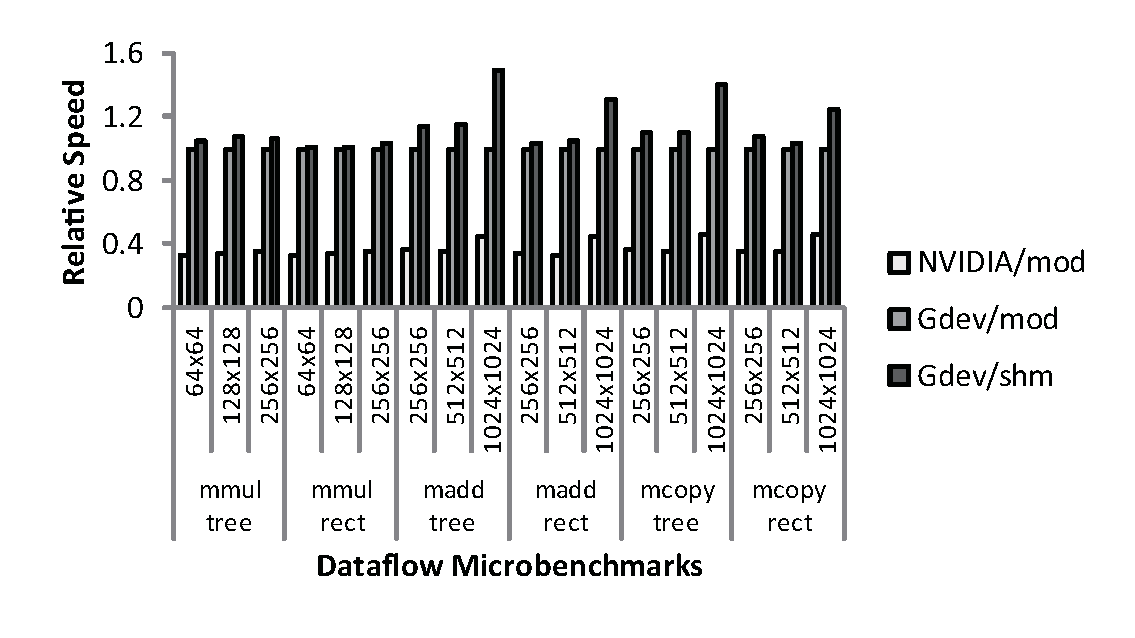
\includegraphics[width=\hsize]{eps/dataflow.eps}\\
  \vspace{-1.5em}
  \caption{Impact of shared memory on dataflow tasks.}
  \label{fig:dataflow}
 \end{center}
 \vspace{-1.5em}
 \begin{center}
  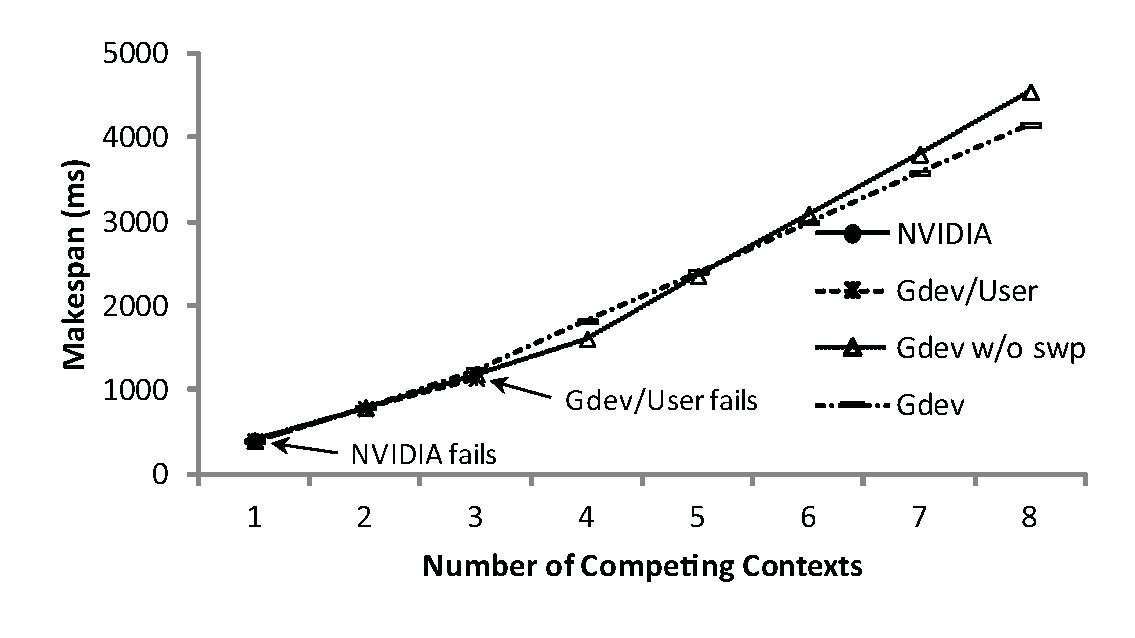
\includegraphics[width=0.8\hsize]{eps/swapping.eps}\\
  \vspace{-1.5em}
  \caption{Impact of swapping latency.}
  \label{fig:swapping}
 \end{center}
 \vspace{-1.5em}
 \begin{center}
  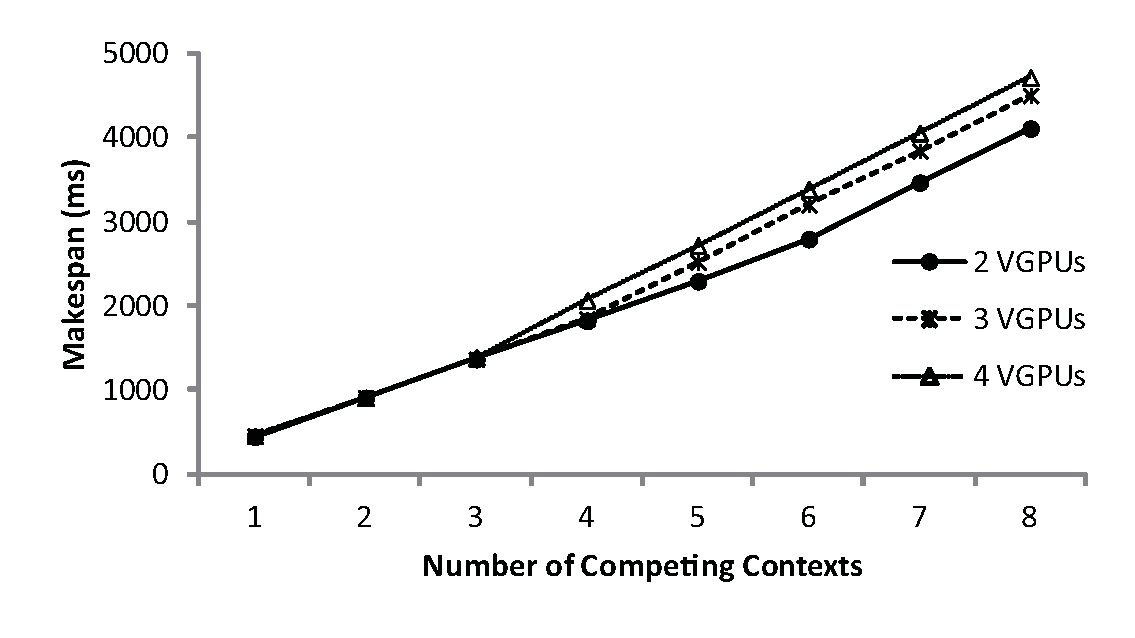
\includegraphics[width=0.8\hsize]{eps/swapping_vgpu.eps}\\
  \vspace{-1.5em}
  \caption{Impact of swapping latency on virtual GPUs.}
  \label{fig:swapping_vgpu}
 \end{center}
 \vspace{-1.5em}
\end{figure}

Figure~\ref{fig:dataflow} shows the speedups of dataflow benchmarks
achieved by using Gdev's shared memory functionality.
We construct a dataflow by either a 6x32 tree or a 6x10 rectangle
graph, respecting PTask's benchmarks~\cite{Rossbach_SOSP11}.
``NVIDIA/modular'' and ``Gdev/modular'' use the vanilla CUDA API
provided by the proprietary software and our Gdev prototype
respectively to implement dataflows in such a way that allocates a
self-contained context to each graph node as a module, and connects
their output and input by copying data between the host and device
memory back and forth.
On the other hand, ``Gdev/shm'' uses shared memory instead of
host-to-device data communication, \textit{i.e.}, it connects the output
and input by sharing the same ``key'' associated with the corresponding
shared memory.
According to the results, the usage of shared memory is very effective
for dataflows with a large size of data, \textit{e.g.}, it gains a 49\%
speedup for the 1024x1024 madd tree.
Specifically, we have observed that ``Gdev/moduler'' took 1424ms while
``Gdev/shm'' took 953ms to complete this dataflow.
This makes sense because the data transfer time for each 1024x1024
integer value was about 8ms on average, and we can reduce data
communications by a total of 32+16+8+4+2=62 intermediate nodes for a
6x32 tree, which leads to a total reduced time of 8x62=496ms.
It is also surprising that our Gdev prototype performs much better than
the proprietary software in this setup.
We suspect that NVIDIA's runtime library takes a long time to initialize
the context when many active contexts co-exist, but a further in-depth
investiation is required.

Figure~\ref{fig:swapping} depicts the impact of memory swapping, enabled
by the Gdev shared memory scheme, on the makespan of multiple 128MB-data
FAST search tasks, where another 1GB-data FAST search task is running at
the highest priority level.
Given that the GeForce GTX 480 used in this evaluation supports
1.6GB of device memory, we cannot create more than three 128MB-data
search tasks at the same time without memory swapping.
``Gdev/User'' hence fails when the number of the small search tasks
exceeds three, since our prototype does not support shared memory in the
user space.
NVIDIA' proprietary software also fails much earlier.
We suspect that it would reserve a large space of device memory for
other purposes.
With memory spapping, however, all the 128MB-data search tasks can
survive to execute under this memory pressure, though the slope of
increase in the makespan changes at a different point when using the
temporal swap space on the device memory under Gdev.
In particular, a reflection point appears clearly when the device swap
space is not leveraged, as observed in ``Gdev w/o swp'', because the
swapping latency influences the makespan.
Using the device swap space, however, Gdev can reduce the impact of
swapping on the makespan, though a reflection point appears a little
earlier due to the swap space itself causing a less total amount of
device memory available for applications.

Figure~\ref{fig:swapping_vgpu} shows the impact of memory swapping on
virtual GPUs.
In this experiment, we introduce virtual GPUs, and execute 128MB-data
search tasks on the first virtual GPU.
The memory size available for the virtual GPU is more restricted in
the presence of more virtual GPUs.
We confirm that the makespans become longer and their refrection points
appear earlier for a greater number of virtual GPUs, but all the search
tasks can still complete.
This explains that memory swapping is also useful on virtual GPUs.

\subsection{Isolation of Virtual GPUs}

\begin{figure*}[t]
 \begin{center}
  \subfigure[FIFO scheduler] {
  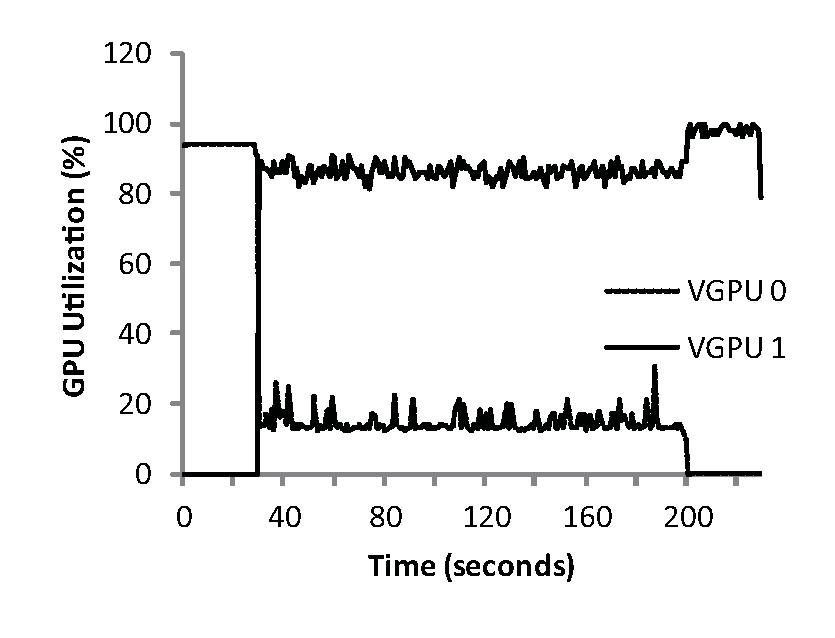
\includegraphics[width=0.319\hsize]{eps/vgpu_2_fifo.eps}
  }
  \subfigure[Credit scheduler] {
  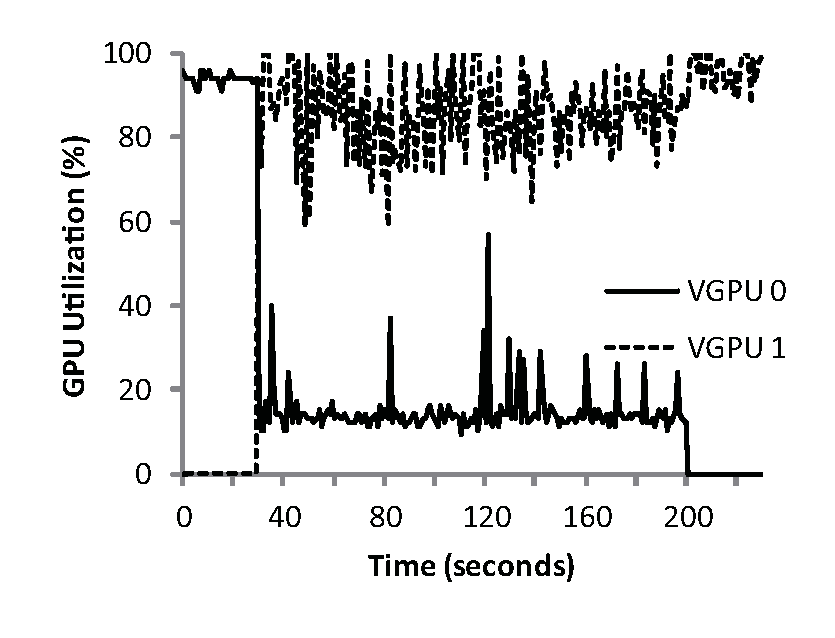
\includegraphics[width=0.319\hsize]{eps/vgpu_2_credit.eps}
  }
  \subfigure[Band scheduler] {
  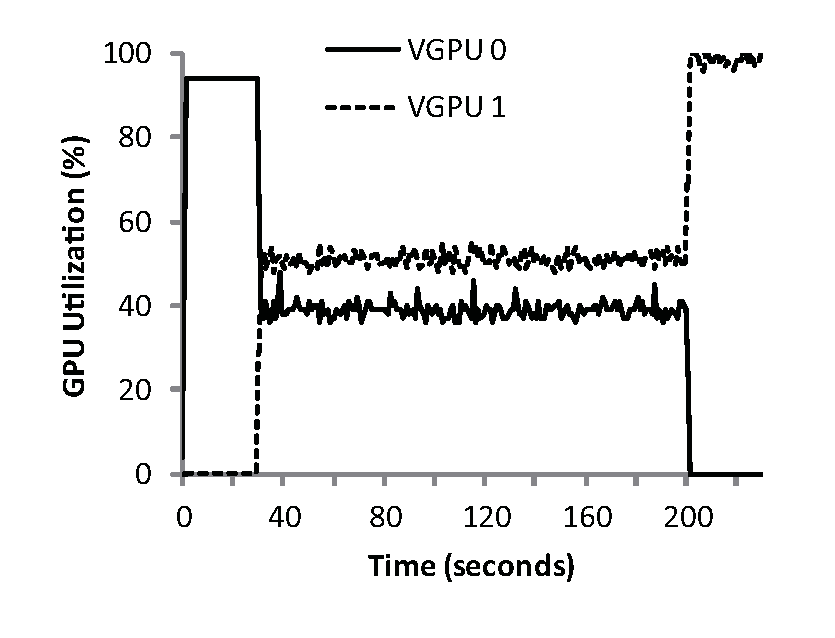
\includegraphics[width=0.319\hsize]{eps/vgpu_2_band.eps}
  }
  \vspace{-1em}
  \caption{Util. of virtual GPUs under extreme workloads.}
  \label{fig:vgpu_2}
  \end{center}
  \vspace{-2em}
\end{figure*}

\begin{figure}[t]
 \begin{center}
  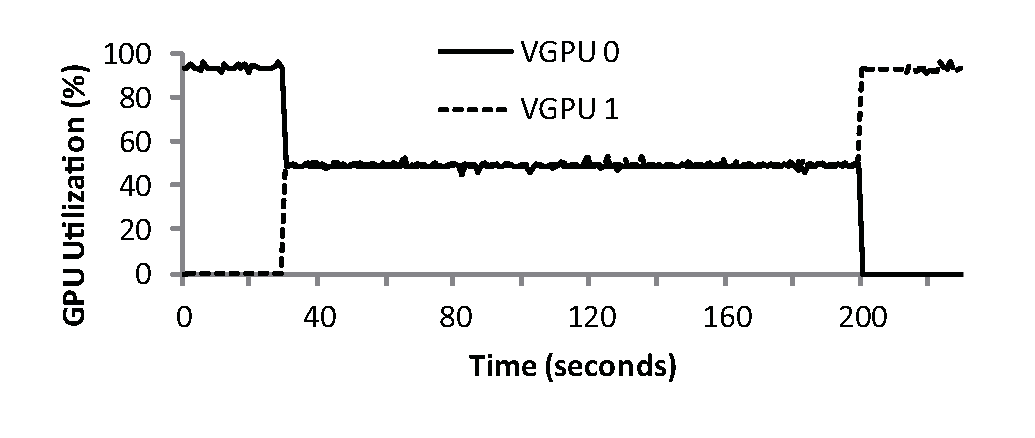
\includegraphics[width=\hsize]{eps/vgpu_fair_2_band.eps}\\
  \vspace{-1.5em}
  \caption{Util. of virtual GPUs under stable workloads.}
  \label{fig:vgpu_fair_2_band}
 \end{center}
 \begin{center}
  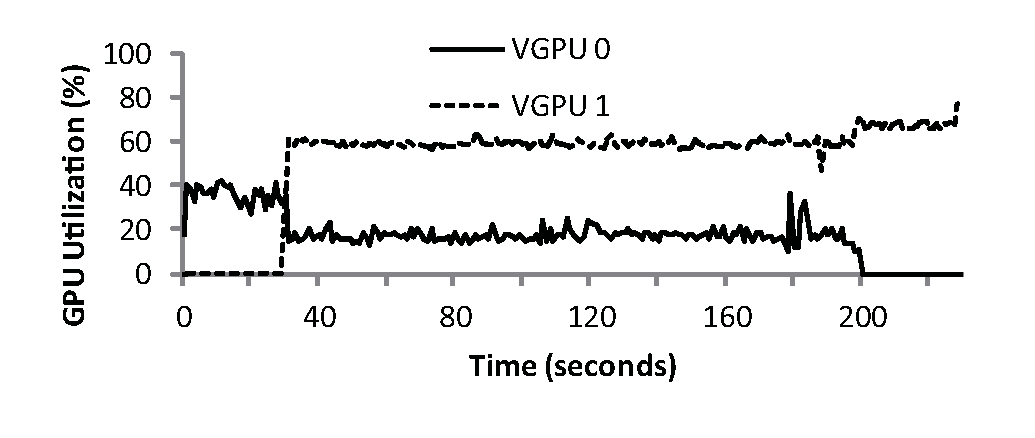
\includegraphics[width=\hsize]{eps/vgpu_2_band_compute.eps}\\
  \vspace{-0.5em}
  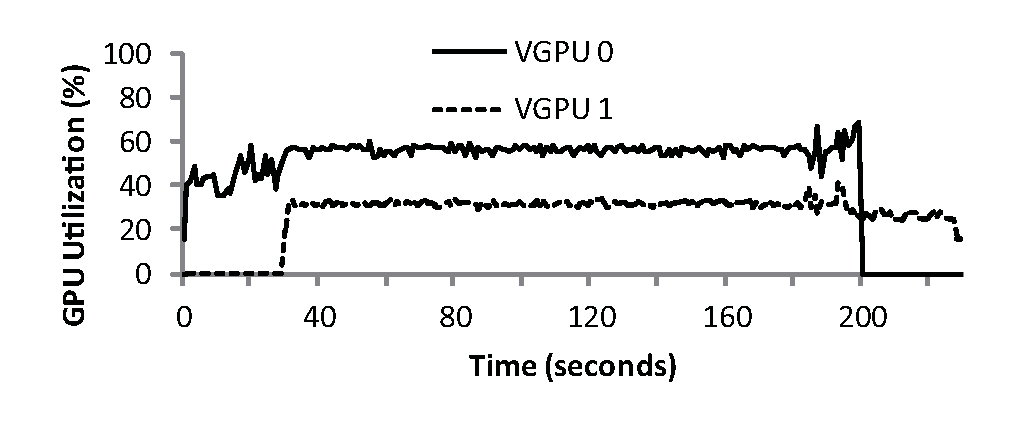
\includegraphics[width=\hsize]{eps/vgpu_2_band_memory.eps}
  \vspace{-1.5em}
  \caption{Util. of virtual GPUs with the MRQ scheme (upper for compute
  and lower for memory bandwidth).}
  \label{fig:vgpu_fair_2_band}
 \end{center}
  \vspace{-2em}
\end{figure}
